\documentclass[12pt]{article}

\title{Activity 2: Arithmetic}
\author{Dr. Chris Mayfield}
\date{CS 149, Fall 2016}

%\ProvidesPackage{cspogil}

% fonts
\usepackage[utf8]{inputenc}
\usepackage[T1]{fontenc}
\usepackage{mathpazo}

% spacing
\usepackage[margin=2cm]{geometry}
\renewcommand{\arraystretch}{1.4}
\setlength{\parindent}{0pt}

% orphans and widows
\clubpenalty=10000
\widowpenalty=10000
\pagestyle{empty}

% figures and tables
\usepackage{graphicx}
\usepackage{multicol}
\usepackage{tabularx}
\usepackage{wrapfig}

% fixed-width columns
\usepackage{array}
\newcolumntype{L}[1]{>{\raggedright\let\newline\\\arraybackslash\hspace{0pt}}m{#1}}
\newcolumntype{C}[1]{>{\centering\let\newline\\\arraybackslash\hspace{0pt}}m{#1}}
\newcolumntype{R}[1]{>{\raggedleft\let\newline\\\arraybackslash\hspace{0pt}}m{#1}}

% include paths
\makeatletter
\def\input@path{{Models/}{../../Models/}}
\graphicspath{{Models/}{../../Models/}}
\makeatother

% colors
\usepackage[svgnames,table]{xcolor}
\definecolor{bgcolor}{HTML}{FAFAFA}
\definecolor{comment}{HTML}{007C00}
\definecolor{keyword}{HTML}{0000FF}
\definecolor{strings}{HTML}{B20000}

% table headers
\newcommand{\tr}{\bf\cellcolor{Yellow!10}}

% syntax highlighting
\usepackage{textcomp}
\usepackage{listings}
\lstset{
    basicstyle=\ttfamily\color{black},
    backgroundcolor=\color{bgcolor},
    numberstyle=\scriptsize\color{comment},
    commentstyle=\color{comment},
    keywordstyle=\color{keyword},
    stringstyle=\color{strings},
    columns=fullflexible,
    keepspaces=true,
    showlines=true,
    showstringspaces=false,
    upquote=true
}

% code environments
\newcommand{\java}[1]{\lstinline[language=java]{#1}}%[
\lstnewenvironment{javalst}{\lstset{language=java,backgroundcolor=}}{}
\lstnewenvironment{javabox}{\lstset{language=java,frame=single,numbers=left}\quote}{\endquote}

% PDF properties
\usepackage[pdftex]{hyperref}
\urlstyle{same}
\makeatletter
\hypersetup{
  pdftitle={\@title},
  pdfauthor={\@author},
  pdfsubject={\@date},
  pdfkeywords={},
  bookmarksopen=false,
  colorlinks=true,
  citecolor=black,
  filecolor=black,
  linkcolor=black,
  urlcolor=blue
}
\makeatother

% titles
\makeatletter
\renewcommand{\maketitle}{\begin{center}\LARGE\@title\end{center}}
\makeatother

% boxes [optional height]
\newcommand{\emptybox}[1][10em]{
\vspace{1em}
\begin{tabularx}{\linewidth}{|X|}
\hline\\[#1]\hline
\end{tabularx}}

% models
\newcommand{\model}[1]{\section{#1}\nopagebreak}
\renewcommand{\thesection}{Model~\arabic{section}}

% questions
\newcommand{\quest}[1]{\subsection*{Questions~ (#1)}}
\newcounter{question}
\newcommand{\Q}{\vspace{1em}\refstepcounter{question}\arabic{question}.~ }
\renewcommand{\thequestion}{\#\arabic{question}}

% sub-question lists
\usepackage{enumitem}
\setenumerate[1]{label=\alph*)}
\setlist{itemsep=1em,after=\vspace{1ex}}

% inline answers
\definecolor{answers}{HTML}{C0C0C0}
\newcommand{\ans}[1]{%
\ifdefined\Student
    \leavevmode\phantom{~~\textcolor{answers}{#1}}
\else
    ~~\textcolor{answers}{#1}
\fi}

% longer answers [optional height]
\newsavebox{\ansbox}
\newenvironment{answer}[1][4em]{
\nopagebreak
\begin{lrbox}{\ansbox}
\begin{minipage}[t][#1]{\linewidth}
\color{answers}
}{
\end{minipage}
\end{lrbox}
\ifdefined\Student
    \phantom{\usebox{\ansbox}}%
\else
    \usebox{\ansbox}%
\fi}


\begin{document}

\maketitle

Now that you've written a few programs, let's take a step back and discuss how to do basic arithmetic.
But first, there's something important to know about why you're working in teams.

\model{Process Skills}

\vspace{-1ex}
\begin{multicols}{2}

\begin{center}
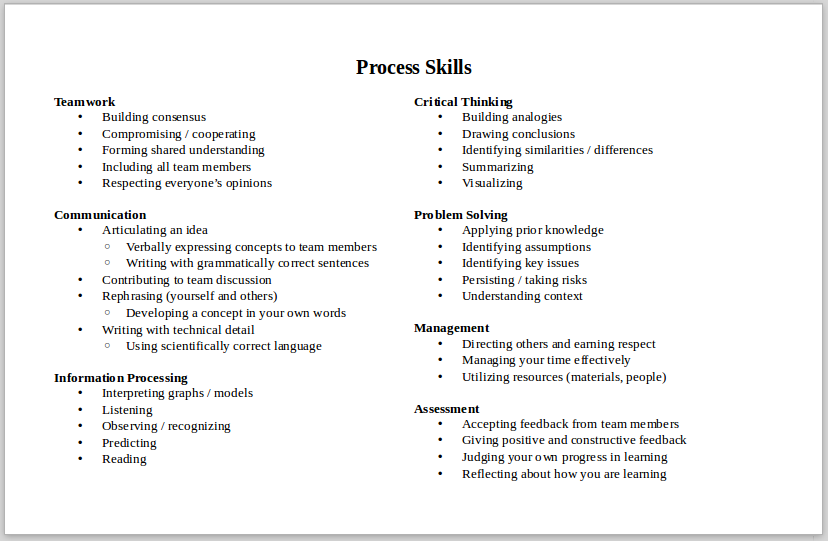
\includegraphics[width=0.8\linewidth]{Meta/process1.png}
\end{center}

\columnbreak
\vspace*{2em}

Your learning team has a new card that is not a role.
It lists the \emph{process skills} that are essential for your ability to construct knowledge.

\end{multicols}


\quest{10 min}


\Q Manager: have each person take turns reading sections of the Process Skills card out loud.
Discuss as a team which skills you would like to focus on today.
Write your top three choices:

\begin{answer}
Teamwork, Problem Solving, Assessment ~ (answers will vary)
\end{answer}


\Q What is a process skill?
As a team, come up with a precise definition.

\begin{answer}
A skill is ``an ability that has been acquired by training'' (WordNet).
Process skills are what you need to learn in college in addition to content.
\end{answer}


\Q What other knowledge and skills do you expect to learn from this course?
How are they different from process skills?

\begin{answer}
Answers may include: how to program, how to debug, and the Java language.
These skills are domain-specific; process skills apply to all disciplines.
\end{answer}


\Q Who has the responsibility to ensure that your team thinks about process skills during the activity each week?
How can the other roles support him/her?

\begin{answer}
The reflector should monitor the teams progress with respect to process skills.
But everyone should self assess and point out examples during the activity.
\end{answer}

% Based on Models 3 and 4 of "Activity 01 Operators" by Helen Hu

\model{Dividing Numbers}
\label{CS1/oper-precedence}

\vspace{-1em}
\begin{center}
\renewcommand{\arraystretch}{1.4}
\begin{tabular}[t]{|C{35pt}|C{65pt}|C{35pt}|}
\hline
 9 / 4 & \textit{evaluates to} & 2 \\
\hline
10 / 4 & \textit{evaluates to} & 2 \\
\hline
11 / 4 & \textit{evaluates to} & 2 \\
\hline
12 / 4 & \textit{evaluates to} & 3 \\
\hline
13 / 4 & \textit{evaluates to} & 3 \\
\hline
14 / 4 & \textit{evaluates to} & 3 \\
\hline
15 / 4 & \textit{evaluates to} & 3 \\
\hline
16 / 4 & \textit{evaluates to} & 4 \\
\hline
\end{tabular}
\hspace{0.5in}
\begin{tabular}[t]{|C{45pt}|C{65pt}|C{45pt}|}
\hline
9    / 4.0 & \textit{evaluates to} & 2.25 \\
\hline
10   / 4.  & \textit{evaluates to} & 2.5 \\
\hline
11.  / 4   & \textit{evaluates to} & 2.75 \\
\hline
12   / 4.0 & \textit{evaluates to} & 3.0 \\
\hline
13   / 4.  & \textit{evaluates to} & 3.25 \\
\hline
14.0 / 4   & \textit{evaluates to} & 3.5 \\
\hline
15   / 4.0 & \textit{evaluates to} & 3.75 \\
\hline
16   / 4.  & \textit{evaluates to} & 4.0 \\
\hline
\end{tabular}
\end{center}


\quest{15 min}

\Q In the first table, which number(s) divided by 4 evaluate to 3?
What is significant about the number of answers you have written down?

\begin{answer}
12, 13, 14, and 15.
There are four answers, and we divided by four.
\end{answer}


\Q How do the answers in the first table differ from the second table?

\begin{answer}
The second table is mathematically correct; the first table rounds down.
\end{answer}


\Q To the right of the second table, round each answer to the closest integer.
How do those values compare to what you see in the first table?

\begin{answer}
The pattern is off by two rows.
The 0.5 and 0.75 values round up, but in the first table they don't.
\end{answer}


\Q Carefully explain the difference between the numbers in the first and second tables.

\begin{answer}
All the numbers in the first table have no decimal points.
At least one number in each row of the second table as a decimal point.
\end{answer}


\Q Complete the table:
\hspace{2em}
\begin{minipage}{0.5\textwidth}
\renewcommand{\arraystretch}{1.4}
\begin{tabular}[t]{|C{45pt}|C{65pt}|C{45pt}|}
\hline
14. / 4. & \textit{evaluates to} & \ans{3.5} \\
\hline
14. / 4  & \textit{evaluates to} & \ans{3.5} \\
\hline
14  / 4. & \textit{evaluates to} & \ans{3.5} \\
\hline
14  / 4  & \textit{evaluates to} & \ans{3}   \\
\hline
\end{tabular}
\end{minipage}


\Q Dividing numbers with fractional parts (known as \textbf{floating-point} numbers) gives you different results from dividing two integers.
In the previous question:

\begin{enumerate}
\item Which rows evaluate to an integer? \ans{the first three}
\vspace{1ex}
\item Which rows evaluate to a floating-point number? \ans{the last one}
\vspace{1ex}
\end{enumerate}


\Q Imagine you are writing a Java program that requires division.

\begin{enumerate}
\item What must be true about the \textbf{operands} (the numbers around the \textbf{operators}) for you to get the mathematically correct answer?

\ans{At least one of them needs to be a floating-point number.}
\vspace{1ex}

\item Does it need to be true for both operands? \ans{No}
\vspace{1ex}
\end{enumerate}


\Q Consider what you know about addition (\java{+}).
If you add two integers in a Java expression, will the result always be mathematically correct?
Justify your answer.

\begin{answer}
Yes, because adding two integers always results in an integer.
(Unless the number gets too large and the arithmetic overflows.)
\end{answer}


\Q What about subtraction (\java{-}) and multiplication (\java{*})? If you subtract or multiply two integers, will the answer always be mathematically correct? Justify your answer.

\begin{answer}
Yes, because subtraction and multiplication can be rewritten in terms of addition.
Division is the only special case, because it has both a quotient and a remainder.
\end{answer}

% Based on Model 1 of "Activity 02 Declaration" by Helen Hu

\model{Variable Declarations}
\label{CS1/variable-declare}

In addition to \textbf{literal} numbers like 1 or 2.3, most Java programs involve \textbf{variables} (named values that can be changed).
The following code \textbf{declares} and \textbf{assigns} three variables:

\begin{javabox}
int dollars;
int cents;
double grams;

dollars = 1;
cents = 90;
grams = 3;
\end{javabox}


\quest{10 min}


\Q Identify the Java \textbf{keyword} used in a variable declaration to indicate

\begin{enumerate}
\item an integer: \ans{int}
\item a floating-point number: \ans{double}
\end{enumerate}


\Q Consider numbers of dollar bills, cents, and grams. Which of these units only makes sense as an integer, and why?

\begin{answer}
Cents makes sense (ha ha) only as an integer, because at the end of the day you can't pay with a fractional amount.
\end{answer}


\Q What would you expect the following statements to print out? (Hint: Refer to \ref{CS1/dividing-numbers}.)

\begin{enumerate}
\item \java{System.out.println(dollars);} \ans{1}
\item \java{System.out.println(cents);} \ans{90}
\item \java{System.out.println(grams);} \ans{3.0}
\end{enumerate}


\Q What do you think the purpose of a variable declaration is?

\begin{answer}
It tells the computer how to interpret and display the value.
\end{answer}


\newpage
\Q Consider the statement: ~ \java{cents = dollars;}

\begin{enumerate}

\item Compare this code to lines 5--7 in \ref{CS1/variable-declare}.
What value do you think cents and dollars will have after running this statement?

\ans{The variable \java{cents} will be 1, and \java{dollars} will remain unchanged.}

\item Which side of the equals sign (left or right) was assigned a new value?
\ans{The left side.}

\end{enumerate}


\Q Examples of Java operators include \java{+} and \java{-}; they describe an operation to be executed (e.g., addition or subtraction).

\begin{enumerate}

\item Do you consider the equals sign in Java an operator (an operation to be executed)?
\\ If so, explain the operation. If not, explain why not.

\ans{Yes; it executes the assignment operation which stores a value in memory.}

\item Do you consider the equals sign in mathematics an operator (an operation to be executed)?
\\ If so, explain the operation. If not, explain why not.

\ans{No; it simply states the proposition that two values are equal.}

\end{enumerate}


\Q In your own words, explain how you should read the \java{=} sign in Java.
For example, the Java statement ~ \java{x = a + b;} ~ should be read as ``x \_\_\_\_\_ a plus b.''

\begin{answer}
Answers may include ``x \emph{gets} a plus b'', ``x \emph{becomes} a plus b'', etc.
\end{answer}

% Based on Model 2 of "Activity 02 Declaration" by Helen Hu

\model{Order of Operations}

The Java language defines a specific order of execution for math and other operations. For example, multiplication and division take \textbf{precedence} over addition and subtraction. Using parentheses, you can override the order of operations.
The following table lists some Java operators from highest precedence to lowest precedence.

\begin{center}
\begin{tabular}{|L{3in}|L{1in}|}
\hline
Parenthesis
& \tt ( ) \\
\hline
Unary (positive or negative signs)
& \tt + - \\
\hline
Multiplicative
& \tt * / \\
\hline
Additive
& \tt + - \\
\hline
Assignment
& \tt = \\
\hline
\end{tabular}
\end{center}

For the following questions, assume you have these two variables:

\begin{javalst}
    int x;
    double y;
\end{javalst}


\quest{10 min}


\Q What operator has the lowest precedence?
Why do you think Java is designed that way?

\begin{answer}
Assignment has the lowest precedence so that all other operations happen first (before the final value is stored in memory).
\end{answer}


\Q The \java{+} and \java{-} operators show up twice in the table of operator precedence.
For the Java expression ~ \java{x = 5 * -3;} ~ explain how you know whether the \java{-} operator is being used as an unary or binary operator in this expression.

\begin{answer}
It matters what is to the left or right of the operator.
In this example, the \java{-} is preceded by a \java{*}, so it must be unary.
\end{answer}


\Q Give the order of operations in the Java expression: ~ \java{x = 5 * -3;}

\begin{enumerate}
\item First operator to be evaluated: \ans{\java{-}}
\item Second operator: \ans{\java{*}}
\item Third operator: \ans{\java{=}}
\end{enumerate}


\Q Give the order of operations in the Java expression: ~ \java{y = 9 / 2;}

\begin{enumerate}
\item First operator to be evaluated: \ans{\java{/}}
\item Second operator: \ans{\java{=}}
\end{enumerate}


\Q Based on your answer to the previous question, explain why the variable \java{y} would be assigned 4.0 (as opposed to 4 or 4.5).

\begin{answer}
If \java{y} is a floating-point variable, the integer result 4 would be stored as 4.0 in memory.
\end{answer}


\Q Rewrite the assignment for \java{y} so that it would be set correctly to 4.5. (Hint: you'll need to recall what you learned about division in \ref{CS1/dividing-numbers}.)

\begin{answer}
\java{y = 9.0 / 2.0;}
\end{answer}


\end{document}
